\chapter{Detailed Report}\label{chapter:detailed_report}

\section{Tool description}

TODO:\newline
compare the 8 different tools used by your team. Which vulnerabilities can each
tool find? Which vulnerabilities can they not find?\newline
Tools generally find a large number of false positives. You must check if the results given to you by tools
are false positives or not. Write in the report what the percentage of false positives are for each tool and
for each type of vulnerability that the tool finds.

\subsection*{Web Testing Tools}

\subsubsection*{devbug.co.uk}
\begin{itemize}
	\item \textbf{Used by}\\ Alexander Lill
	\item \textbf{Used for}\\
	DevBug is a basic PHP Static Code Analysis (SCA) tool written mostly in JavaScript. The idea behind DevBug is to make basic PHP Static Code Analysis accessible online, to raise security awareness and to integrate SCA into the development process. DevBug can be used to quickly test a page of PHP that you think may have some potential vulnerabilities, to run across a piece of code you have found on Google that you are unsure of or to directly write your own code in.
	
	This tool was used as an additional resource for Static Code Analysis reports.
	
	The website shows e.g. Cross-Site-Scripting and Command Injection vulnerabilities.
	\item \textbf{Useful in}\\ \vulnref{OTG-INPVAL-001} and \vulnref{OTG-INPVAL-002}
\end{itemize}

\subsubsection*{Kiuwan}
\begin{itemize}
	\item \textbf{Used by}\\ Alexander Lill
	\item \textbf{Used for}\\
	Kiuwan (see \url{https://www.kiuwan.com}) is a software as a service (SaaS) static program analysis multi-technology software for software analytics, quality and security measurement and management.
	
	This tool was used as a main source for possible vulnerabilities using Static Code Analysis.
	
	The tool shows defects in the categories "Maintainability", "Security", "Efficiency","Portability" and "Reliability" (see \autoref{figure:kiuwan}) as well as estimates for the effort to fix those issues. It can be connected with e.g. Github and automatically analyzes the code after every commit and shows metrics.
	\item \textbf{Useful in}\\ \vulnref{OTG-INPVAL-001} and \vulnref{OTG-INPVAL-002}
\end{itemize}

\begin{figure}[h!tbp]
	\centering
	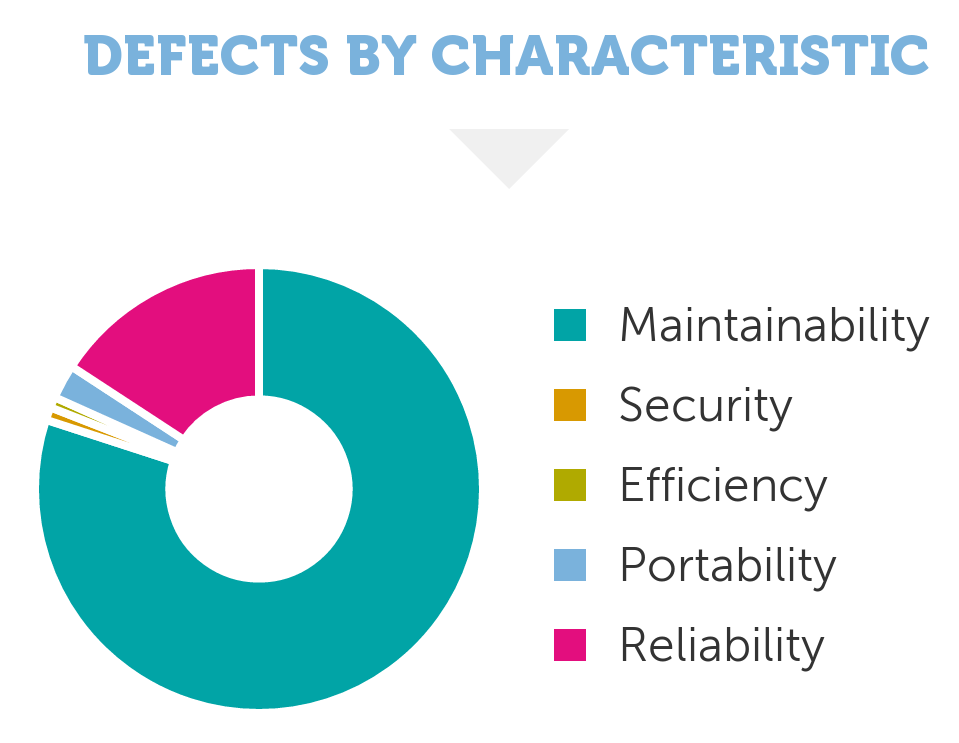
\includegraphics[width=0.5\textwidth]{figures/kiuwanResults}
	\caption{Example graph from Kiuwan}
	\label{figure:kiuwan}
\end{figure}

\subsubsection*{RIPS}
\begin{itemize}
	\item \textbf{Used by}\\ Name Surname
	\item \textbf{Used for}\\ Sample Text - description of the tool
	\item \textbf{Useful in}\\ \vulnref{OTG-AUTHN-004} and \vulnref{OTG-AUTHN-005}
\end{itemize}

\subsubsection*{RATS}
\begin{itemize}
	\item \textbf{Used by}\\ Name Surname
	\item \textbf{Used for}\\ Sample Text - description of the tool
	\item \textbf{Useful in}\\ \vulnref{OTG-AUTHN-004} and \vulnref{OTG-AUTHN-005}
\end{itemize}

\subsubsection*{Comparison}
TODO: Comparison Text


\subsection*{C and Java Testing Tools}

\subsubsection*{IDA Pro}
\begin{itemize}
	\item \textbf{Used by}\\ Name Surname
	\item \textbf{Used for}\\ Sample Text - description of the tool
	\item \textbf{Useful in}\\ \vulnref{OTG-AUTHN-004} and \vulnref{OTG-AUTHN-005}
\end{itemize}

\subsubsection*{Radare2}
\begin{itemize}
	\item \textbf{Used by}\\ Name Surname
	\item \textbf{Used for}\\ Sample Text - description of the tool
	\item \textbf{Useful in}\\ \vulnref{OTG-AUTHN-004} and \vulnref{OTG-AUTHN-005}
\end{itemize}

\subsubsection*{JAVA Decompiler}
\begin{itemize}
	\item \textbf{Used by}\\ Name Surname
	\item \textbf{Used for}\\ Sample Text - description of the tool
	\item \textbf{Useful in}\\ \vulnref{OTG-AUTHN-004} and \vulnref{OTG-AUTHN-005}
\end{itemize}

\subsubsection*{Comparison}
TODO: Comparison Text

\clearpage

TODO:\newline
describe identified vulnerabilities mentioning the following for each one
\begin{itemize}
	\item Observation: which part of the application is vulnerable and why?
	\item Discovery: how was this vulnerability discovered? Which tools were used and which steps were performed?
	\item Likelihood: what is the likelihood that this vulnerability is exploited? Which assumptions must hold and which skills must an attacker have?
	\item Impact: what is the potential impact of an exploit of this vulnerability? What could happen?
	\item Recommendation: how exactly would you fix this problem?
	\item Instantiate the CVSS v3.0 template for this particular vulnerability.
	\item Comparison with your own application: how and why is your app better/worse
\end{itemize}

NOTR: Each vulnerability should be described on a new page!\newline

\clearpage
%Sample tables
\vultable{\bs}{%
	Observation: which part of the application is vulnerable and why?
}{%
	Discovery: how was this vulnerability discovered? Which tools were used and which steps were performed?
}{%
	Likelihood: what is the likelihood that this vulnerability is exploited? Which assumptions must hold and which skills must an attacker have?
}{%
	Impact: what is the potential impact of an exploit of this vulnerability? What could happen?
}{%
	Recommendation: how exactly would you fix this problem?
}{%
	\na
	%\secure
	%\cvssBaseScorePretty{N}{H}{N}{R}{U}{H}{H}{N}
}
\vultable{\gnb}{%
	Observation: which part of the application is vulnerable and why?
}{%
	Discovery: how was this vulnerability discovered? Which tools were used and which steps were performed?
}{%
	Likelihood: what is the likelihood that this vulnerability is exploited? Which assumptions must hold and which skills must an attacker have?
}{%
	Impact: what is the potential impact of an exploit of this vulnerability? What could happen?
}{%
	Recommendation: how exactly would you fix this problem?
}{%
	\na
	%\secure
	%\cvssBaseScorePretty{N}{H}{N}{R}{U}{H}{H}{N}
}
Comparison with your own application: how and why is your app better/worse
\clearpage

\section{Configuration and Deploy Management Testing}
\simpleVulntitle{OTG-CONFIG-003}{Test File Extensions Handling for Sensitive Information}
\vultable{\bs}{%
	We discovered that it is possible to access some files and directories which should not be accessible to the user/attacker. Specifically, we were able to get a hold of the private key used by the server for SSL encryption, the MySQL dump file and other data that should not be accessible from the network and, even less, to attackers.
}{%
	We managed to directly download several files containing sensitive information directly, as well as access some unprotected content:
	\begin{itemize}
		\item \texttt{http://[HOST]/app/HTTPS/hostonly.key}
		\item \texttt{http://[HOST]/adminer}
		\item \texttt{http://[HOST]/dump.sql}
		\item \texttt{http://[HOST]/Smart-Card-Simulator/src/scs/Main.java}, as well as all other Java sources.
	\end{itemize}
	Also many other README and temporary files are directly accessible.\newline
}{%
	Since directory listing is disabled inside the /api and /app subfolders of the application, most of the mentioned files can be accessed only via brute-force attacks, and even then it would prove very difficult to guess the name of the directory and filename correctly. During white-box testing, this was not an issue, but in reality, finding out this weakness would require many attempts and much time.\newline
	Other names of files, however, contained in the root folder (directory listing here is not disabled), like dump.sql can be easily guessed.
}{%
	Although an attacker cannot directly compromise the integrity and availability of the server, it is possible to access some very important content of the application. In particular, getting a hold of \texttt{hostonly.key} allows to start MITM attacks on any victim, since the file contains the private key of the server used for SSL encryption.
}{%
	Relocate the .htaccess files (or the root of the web application) and place more strict rules for file/directory access, since these are too loose.
}{%
	\cvssBaseScorePretty{N}{H}{N}{N}{U}{H}{N}{N}
}
\vultable{\gnb}{%
	TODO: Observation
}{%
	TODO: Discovery
}{%
	TODO: Likelihood
}{%
	TODO: Implications
}{%
	TODO: Recommendation
}{%
	\naScore
}

\vulntitle{OTG-CONFIG-006}{Test HTTP Methods}
\vulntitle{OTG-CONFIG-007}{Test HTTP Strict Transport Security}
\vultable{\bs}{%
	Although HTTPS is enabled on port 443, access to the page without using HTTPS is still possible, by simply accessing the server on port 80. However, since this was left on purpose by the developers for testing purposes, we decided not to treat this as a vulnerability (no CVSS score is given).
}{%
	This information was given to us directly by the Team that developed the Bank System application. We also proved this by simply trying to access the application on port 80: this way we had normal access to the application, although without any transport security.
}{%
	Since we are not considering this as a vulnerability, we won't analyze it in depth.
}{%
	The implications of lack of an encrypted connection were already analysed in phase 2. Since we are not considering this as a vulnerability anyway, we won't analyze its implications.
}{%
	Redirect any requests from port 80 to port 443. This is highly recommended before the application goes live.
}{%
	\secure
}
\vultable{\gnb}{%
	This vulnerability was fixed in phase 3 and the application is only allowing communication between the client and the server via HTTPS.
}{%
	We discovered this by simply testing to access both ports 80 and 443 on the webserver, which only allowed us to connect to the latter. A connection on port 80 was refused by the server. We also enforced this theory by checking it with nmap, getting the same result.
}{%
	\na
}{%
	\na
}{%
	\na
}{%
	\secure
}

\vulntitle{OTG-CONFIG-008}{Test RIA cross domain policy}

\clearpage
\section{Identity Management Testing}
\simpleVulntitle{OTG-IDENT-001}{Test Role Definitions}
\vultable{\bs}{%
	The role definitions are implemented as specified in their report for phase 2 and are secure.
}{%
	Manual testing and checking the contraints in the source code, e.g. \texttt{api/index.php}
}{%
	\na
}{%
	\na
}{%
	\na
}{%
	\secure
}
\vultable{\gnb}{%
	\same
}{%
	Manual testing and checking the contraints in the source code, e.g. \texttt{db.php}
}{%
	\na
}{%
	\na
}{%
	\na
}{%
	\secure
}



\vulntitle{OTG-IDENT-002}{Test User Registration Process}
\vultable{\bs}{%
	The registration process is set up for anyone to register, the process then awaits human interaction for the approval stage, this will serve an extra step of verification. Mail addresses have to be unique and can not be used by multiple users.
	
	Identities are not verified nor checked at this stage due to application limitations.
	
	No CAPTCHA or similar tests available to test if users are robots or human.
}{%
	Manual testing and checking the source code if duplicate mail addresses are possible. Here the database prevents the entry of a duplicate mail address, while the front end shows "Registration successful. Waiting for approval. You will be notified to email." even if the mail address was already in the dabase and the new account not successfully created.
}{%
	High. It is easy to create a lot of new users as long as a syntactically valid mail address is provided.
}{%
	Medium. A lot of new users could lead to performance or availability problems in the database. These registered users can not be used on the website as long as they are not approved, though.
}{%
	The introduction of CAPTCHAs, any other check for human users or some invitation mechanism might solve this issue.
}{%
	TODO: Score
}
\vultable{\gnb}{%
	\same
}{%
	Manual testing and checking the source code if duplicate mail addresses are possible. Here the database prevents the entry of a duplicate mail address and shows a message upon registration if the mail address was already used.
}{%
	\na
}{%
	\na
}{%
	\na
}{%
	TODO: Score
}

\vulntitle{OTG-IDENT-003}{Test Account Provisioning Process}
\vultable{\bs}{%
	Provisioning clients is an easy process with no effective mechanisms
to verify or vet clients besides a manual approval process, provisioning employees is set up in a similar matter.
Vulnerabilities with creating the client account have been discussed
in the previous section \vulnref{OTG-IDENT-002}, the same applies to creating
employee accounts, so a potential DOS attack is possible by creating
robot accounts.
}{%
	This was found through following the given process for creating
accounts.
}{%
	High. It is easy to create a lot of new users as long as a syntactically valid mail address is provided.
}{%
	Medium. A lot of new users could lead to performance or availability problems in the database. These registered users can not be used on the website as long as they are not approved, though.
}{%
	The introduction of CAPTCHAs, any other check for human users or some invitation mechanism might solve this issue.
}{%
	TODO: Score
}
\vultable{\gnb}{%
	\same
}{%
	\same
}{%
	\same
}{%
	\same
}{%
	\same
}{%
	TODO: Score
}

\vulntitle{OTG-IDENT-004}{Testing for Account Enumeration and Guessable User Account}
\vultable{\bs}{%
	The user account names are the users mail addresses and therefore not easily guessable. The \bs{} is vulnerable for Account Enumeration: Logins with an associated mail address and a wrong password lead to the message "Incorrect data. Wrong user or password. You have X tries more.", while a login with an unassociated mail address and any password leads to the message "Incorrect data. Wrong user or password".
}{%
	This was discovered manually in the source code (file \texttt{api/index.php} lines 178-180 and 214-245) and confirmed by manual testing.
}{%
	The use of this vulnerability is very likely as this is a very easy way to get to know valid user accounts.
}{%
	This vulnerability has a high impact as many more advanced attacks are possible as soon as valid mail addresses for the login are known.
}{%
	We recommend to always show the same error message, even though the user does not see how many tries he still has left.
}{%
	TODO: Score
}
\vultable{\gnb}{%
	The \gnb{} application is always showing the same error message and is thus not vulnerable. We do also use the users mail address as user account names which makes them not easily guessable.
}{%
	\na
}{%
	\na
}{%
	\na
}{%
	\na
}{%
	\secure
}

\vulntitle{OTG-IDENT-005}{Testing for Weak or unenforced username policy}
\vultable{\bs}{%
	Username has to be in valid email address format.
}{%
	This was found through trial and error and checking the according files (e.g. \texttt{index.php}, line 483).
}{%
	\na
}{%
	\na
}{%
	\na
}{%
	\secure
}
\vultable{\gnb}{%
	\same
}{%
	This was found through trial and error and checking the according files (e.g. \texttt{js/registration.js} line 81, \texttt{registration/registration\_request.php} line 29).
}{%
	\same
}{%
	\same
}{%
	\same
}{%
	\secure
}

\clearpage
\section{Authentication Testing}
\simpleVulntitle{OTG-AUTHN-001}{Testing for Credentials Transported over an Encrypted Channel}
\vulntitle{OTG-AUTHN-002}{Testing for default credentials}
\vultable{\bs}{%
	The developers left a temporary administrator test account with weak credentials. It is likely that this was done specifically for testing purposes, but we decided to treat this as a vulnerability anyway, since this should be avoided when the application goes live.\newline
	This flaw aside, no other accounts with weak credentials were found; also passwords are not automatically generated for users and the password policy is strict, not allowing weak passwords or empty fields for that matter.
}{%
	The default credentials left for testing purposes were:\newline
	\texttt{user: test4@test.org pass: test}\newline
	These were given to us directly by the developers. To prove our point, we also searched through the Rocktyou.txt password list (found at \texttt{https://wiki.skullsecurity.org/index.php?title=Passwords} and proved that 'test' is a very weak password.
}{%
	The likelihood of cracking the password is high. Brute-forcing the username may require some more effort, but since the application returns different error codes depending whether the inserted username or password were wrong, an attacker can easily try out any possible username.
}{%
	In this particular case the implications are severe, since a successful attack would grant an attacker admin rights, with consequent full access to the application.
}{%
	It is highly recommended to change the default credentials of the application admin before deploying the application.
}{%
	\cvssBaseScorePretty{N}{L}{L}{N}{U}{L}{N}{H}
}

\vultable{\gnb}{%
	The same observations made for Bank System apply. Furthermore, no weak default credentials were left at all (not even for testing purposes).
}{%
	\na
}{%
	\na
}{%
	\na
}{%
	\na
}{%
	\secure
}


\vulntitle{OTG-AUTHN-003}{Testing for Weak lock out mechanism}
\vulntitle{OTG-AUTHN-004}{Testing for bypassing authentication schema}
\vulntitle{OTG-AUTHN-005}{Test remember password functionality}
\vulntitle{OTG-AUTHN-006}{Testing for Browser cache weakness}
\vultable{\bs}{%
	We observed that no Browser cache weaknesses could be exploited for this web application. This statement only holds when HTTPS is enforced (see \vulnref{OTG-CONFIG-007}). It is important to stress though, that the Bank System application does not explicitly avoid cache weaknesses, as can be seen in any intercepted server response. This is not a problem, however, since the used Framework dynamically loads the sensitive information of the page using asynchronous Ajax requests, which are not cached by the browser.
}{%
	Browser history was tested manually, showing no issues.\newline 
	The browser cache was tested using the CacheViewer2 addon for Firefox: this showed us that server responses are actually cached by the browser, but these are encrypted as long as HTTPS is used. Also, given that Bank System dynamically loads pages, we only managed to restore some pages from the cache.
}{%
	\na
}{%
	\na
}{%
	Although the application didn't show evident browser cache weaknesses, it is still recommended to set some additional cache-control: no-cache, no-store, must-revalidate.
}{%
	\secure
}

\vultable{\gnb}{%
	The GNB application enforces cache invalidation, preventing the browser from storing any sensible information other that stylesheets and javascript files locally. Browser history also couldn't be exploited, since the application delivers the pages over HTTPS.
}{%
	Browser history was tested manually, showing no issues. Browser cache was tested using the CacheViewer2 addon for Firefox. We also analyzed some responses from the server, only to see that the application sets the following flags:\newline
	\texttt{Cache-Control: private, must-revalidate}
}{%
	\na
}{%
	\na
}{%
	\na
}{%
	\secure
}
\vulntitle{OTG-AUTHN-007}{Testing for Weak password policy}
\vulntitle{OTG-AUTHN-008}{Testing for Weak security question/answer}
\vultable{\bs}{%
	\notImp
}{%
	\na
}{%
	\na
}{%
	\na
}{%
	\na
}{%
	\na
}
\vultable{\gnb}{%
	\notImp
}{%
	\na
}{%
	\na
}{%
	\na
}{%
	\na
}{%
	\na
}

\vulntitle{OTG-AUTHN-009}{Testing for weak password change or reset functionalities}
\vulntitle{OTG-AUTHN-010}{Testing for Weaker authentication in alternative channel}

\clearpage
\section{Authorization Testing}
\simpleVulntitle{OTG-AUTHZ-001}{Testing Directory traversal/file include}
\vulntitle{OTG-AUTHZ-002}{Testing for bypassing authorization schema}
\vultable{\bs}{%
	No vulnerabilities in this area were found for the \bs{} application.
}{%
	This was observed by checking all necessary functions in the file \texttt{api/index.php} which does all the checks if a request is valid or not and some manual trial and error testing.
}{%
	\na
}{%
	\na
}{%
	\na
}{%
	\secure
}
\vultable{\gnb}{%
	No vulnerabilities in this area were found for the \gnb{} application.
}{%
	This was observed by checking all necessary functions in the according files and some manual trial and error testing.
}{%
	\na
}{%
	\na
}{%
	\na
}{%
	\secure
}

\vulntitle{OTG-AUTHZ-003}{Testing for Privilege Escalation}
\vulntitle{OTG-AUTHZ-004}{Testing for Insecure Direct Object References}

\clearpage
\section{Session Management Testing}
\simpleVulntitle{OTG-SESS-001}{Testing for Bypassing Session Management Schema}
\vulntitle{OTG-SESS-002}{Testing for Cookies attributes}

\vultable{\bs}{%
	We observed that the \bs{} application is not setting all possible cookie attributes, see \autoref{table:cookieattributes}.
}{%
	This was discovered using manual examination of the cookies and additionally by checking the source code for cookie settings.
}{%
	The likelihood is quite high for the exploitation of the missing "HTTP only" and "secure" attributes. The missing "secure" attribute could be related to \vulnref{OTG-CONFIG-007}.
}{%
	This could have a quite big impact as Cookies could be transferred over an insecure connection. Additionally cookies can be read using Javascript e.g. by XSS vulnerabilities.
}{%
	We recommend to set the missing cookie attributes accordingly.
}{%
	TODO: Score
}

\vultable{\gnb}{%
	The \gnb{} application is setting all necessary and/or useful cookie attributes, see \autoref{table:cookieattributes}.
}{%
	\same
}{%
	\na
}{%
	\na
}{%
	\na
}{%
	\secure
}

\begin{table}
\centering
\begin{tabular}{| l | p{3cm} | p{3cm} |}
Attribute & 	\bs{} & \gnb{} \\
\toprule
Session & 		yes	& yes \\
\midrule
Host only &		yes	& yes \\
\midrule
HTTP only &		no	& yes \\
\midrule
Secure &		no	& yes \\
\midrule
Expiry date &	\multicolumn{2}{c|}{Not necessary because of "session" attribute} \\
\bottomrule

\end{tabular}
\caption{Cookies attributes}
\label{table:cookieattributes}
\end{table}

\vulntitle{OTG-SESS-003}{Testing for Session Fixation}
\vulntitle{OTG-SESS-004}{Testing for Exposed Session Variables}
\vulntitle{OTG-SESS-005}{Testing for Cross Site Request Forgery}
\vulntitle{OTG-SESS-006}{Testing for logout functionality}
\vultable{\bs}{%
	We observed that the logout can be easily circumvented by just re-creating the old cookies with the same values before the logout. That means that we can easily undo the logout by just adding a cookie locally.
}{%
	We discovered this by manually looking through the source code and confirmed this by manual testing. \autoref{lst:logoutbug} shows the bug that makes this exploit possible. The variable \texttt{\$UserId} in line 15 is not defined in this context. leading to an SQL \texttt{UPDATE} statement with the following invalid \texttt{WHERE} clause: \texttt{where UserId='';}.
}{%
	It is very likely that this vulnerability will be exploited as cookies can be stolen quite easy (see \vulnref{OTG-SESS-002}) and this removes the timing aspect of stealing a given session. Logging out from the users session does not prevent any further attacks for this session.
}{%
	The potential impact of this vulnerability is high as this makes stealing a user's session much easier. An attacker only needs to get access to the users PHPSESSID or the not completely secure cookie.
}{%
	This issue can be easily resolved by using \texttt{\$user->UserId} instead if the undefined \texttt{\$UserId}.
}{%
	TODO: Score
}

\begin{minipage}{\linewidth}
\begin{lstlisting}[language=PHP, label={lst:logoutbug}, numbers=left, caption=Logout Bug]
    $app->get('/logout', function() use ($app, $db, $queries) {
        csrf_check();
        $user = getCurrentUserInfo();
        session_start();
        if (isset($_COOKIE['PHPSESSID'])) {
            setcookie('PHPSESSID', '', time() - 3600, '/');
        }
        if (isset($_COOKIE['XSRF-TOKEN'])) {
            setcookie('XSRF-TOKEN', '', time() - 3600, '/');
        }
        session_unset();   // Remove the $_SESSION variable information.
        session_destroy();// Remove the server-side session information.
        $query = $queries["updateSessionId"]();
        $statement = getStatement($query);
        $statement->bind_param('si', $sessionId, $UserId);
        $sessionId=NULL;
        $statement->execute();
        $statement->store_result();
    });
\end{lstlisting}
\end{minipage}

\vultable{\gnb}{%
	No vulnerabilities in the logout mechanism have been found in the \gnb{} application.
}{%
	\same
}{%
	\na
}{%
	\na
}{%
	\na
}{%
	\na
}

\vulntitle{OTG-SESS-007}{Test Session Timeout}
\vulntitle{OTG-SESS-008}{Testing for Session puzzling}

\clearpage
\section{Data Validation Testing}
\simpleVulntitle{OTG-INPVAL-001}{Testing for Reflected Cross Site Scripting}
\vultable{\bs}{%
	No Reflected Cross Site Scripting vulnerabilities have been found in the \bs{} application. There is only one place where user input is directly echoed onto a website, but this happens in the API (see \texttt{api/index.php} line 142) and is thus not visible.
}{%
	This was discovered by checking the results of RIPS (which only showed false positives), the results of \url{http://devbug.co.uk} and manually testing a few functionalities.
}{%
	\na
}{%
	\na
}{%
	\na
}{%
	\secure
}

\vultable{\gnb}{%
	No Reflected Cross Site Scripting vulnerabilities have been found in the \bs{} application. There is no place where user input is directly shown on any site.
}{%
	This was discovered by checking the results of RIPS (which only showed false positives), the results of \url{http://devbug.co.uk} and manually testing a few functionalities.
}{%
	\na
}{%
	\na
}{%
	\na
}{%
	\secure
}

\vulntitle{OTG-INPVAL-002}{Testing for Stored Cross Site Scripting}
\vultable{\bs}{%
	No Stored Cross Site Scripting vulnerabilities have been found in the \bs{} application.
}{%
	This was discovered by checking the results of RIPS (which only showed false positives), the results of \url{http://devbug.co.uk} and manually testing a few functionalities.
	
	The \bs{} application is using the AngularJS framework (see \url{https://angularjs.org}) which also includes input sanitization (see \url{https://docs.angularjs.org/api/ngSanitize/service}).
}{%
	\na
}{%
	\na
}{%
	\na
}{%
	\secure
}

\vultable{\gnb}{%
	No Stored Cross Site Scripting vulnerabilities have been found in the \bs{} application.
}{%
	This was discovered by checking the results of RIPS (which only showed false positives), the results of \url{http://devbug.co.uk} and manually testing a few functionalities.
	
	The \gnb{} application is not using any frameworks but instead implemented its own input sanitization (see \texttt{genericfunctions.php} lines 10-103.
}{%
	\na
}{%
	\na
}{%
	\na
}{%
	\secure
}

\vulntitle{OTG-INPVAL-003}{Testing for HTTP Verb Tampering}
\vulntitle{OTG-INPVAL-004}{Testing for HTTP Parameter pollution}
\vulntitle{OTG-INPVAL-005}{Testing for SQL Injection}
\vulntitle{OTG-INPVAL-006}{Testing for LDAP Injection}
\vulntitle{OTG-INPVAL-007}{Testing for ORM Injection}
\vulntitle{OTG-INPVAL-008}{Testing for XML Injection}
\vulntitle{OTG-INPVAL-009}{Testing for SSI Injection}
\vulntitle{OTG-INPVAL-010}{Testing for XPath Injection}
\vulntitle{OTG-INPVAL-011}{IMAP/SMTP Injection}
\vulntitle{OTG-INPVAL-012}{Testing for Code Injection}
\vulntitle{OTG-INPVAL-012-1}{Testing for Local File Inclusion}
\vultable{\bs}{%
	No Local File Inclusion vulnerabilities have been found in the \bs{} application.
}{%
	This was discovered by checking the results of RIPS (which only showed false positives) and checking a few files manually.
}{%
	\na
}{%
	\na
}{%
	\na
}{%
	\secure
}

\vultable{\gnb}{%
	\same
}{%
	\same
}{%
	\na
}{%
	\na
}{%
	\na
}{%
	\secure
}

\vulntitle{OTG-INPVAL-012-2}{Testing for Remote File Inclusion}
\vultable{\bs}{%
	No Remote File Inclusion vulnerabilities have been found in the \bs{} application.
}{%
	This was discovered by checking the results of RIPS (which only showed false positives) and checking a few files manually.
}{%
	\na
}{%
	\na
}{%
	\na
}{%
	\secure
}

\vultable{\gnb}{%
	\same
}{%
	\same
}{%
	\na
}{%
	\na
}{%
	\na
}{%
	\secure
}

\vulntitle{OTG-INPVAL-013}{Testing for Command Injection}
\vultable{\bs}{%
	We observed that it is possible to perform command injection attacks, by exploiting the batch transaction functionality, 
	as no input validation upon the values inserted by the user in the transaction description field is performed. \newline
	Regardless of the type of used banking method (either SCS or pre-generated TANs), as long as a user inserts a valid TAN when performing a transaction, it will also be possible to inject commands to the target system through the description field.
}{%
	This was discovered while analyzing the \texttt{uploadFile} callback function in the index.php file (lines 95-154).\newline
	Since the application doesn't sanitize user input (neither on client nor on server side), the \texttt{exec} function called from the server to execute the C parser can be exploited to execute arbitrary commands, by simply inserting them into the description field. These commands will simply be executed after the parser. Here is an example:\newline
	\texttt{test"; ls -l; exit 1 \#} \newline
	\textbf{Note:} since the output of the \texttt{exec} operation is only visible on client side if the return code was different than 0 (hence on transaction failure), we just need to force a return code (as shown in the example above).
}{%
	This kind of attack may require several brute-force attempts and has therefore medium likelihood, but once found out, the vulnerability is easy to exploit.
}{%
	The implications of this attack are high, since the attacker is able to execute arbitrary commands on the target system. It is important to stress though, that it is not possible to modify any file in the target web directory, due to insufficient privileges.
}{%
	It is highly recommended to sanitize the description value inserted by the user, or to make the user write the descriptions directly inside the batch file, avoiding thus command injections.
}{%
	\cvssBaseScorePretty{N}{L}{L}{N}{U}{L}{N}{H}
}
\vultable{\gnb}{%
	Observation
}{%
Discovery
}{%
Likelihood
}{%
Implications
}{%
Recommendation
}{%
\naScore
%\cvssBaseScorePretty{N}{H}{N}{R}{U}{H}{H}{N}
}

\vulntitle{OTG-INPVAL-014}{Testing for Buffer overflow}
\vulntitle{OTG-INPVAL-014-2}{Testing for Stack overflow}
\vulntitle{OTG-INPVAL-014-3}{Testing for Heap overflow}
\vulntitle{OTG-INPVAL-014-4}{Testing for Format string}
\vulntitle{OTG-INPVAL-015}{Testing for incubated vulnerabilities}
\vulntitle{OTG-INPVAL-016}{Testing for HTTP Splitting/Smuggling}
This vulnerability was not tested as we did not extend our testing to the Apache Web Server.

\clearpage
\section{Error Handling}
\simpleVulntitle{OTG-ERR-001}{Analysis of Error Codes}
\vulntitle{OTG-ERR-002}{Analysis of Stack Traces}

\clearpage
\section{Cryptography}
\simpleVulntitle{OTG-CRYPST-001}{Testing for Weak SSL/TSL Ciphers, Insufficient Transport Layer Protection}
\vulntitle{OTG-CRYPST-002}{Testing for Padding Oracle}
\vultable{\bs}{%
	\notImp
}{%
	\na
}{%
	\na
}{%
	\na
}{%
	\na
}{%
	\na
}
\vultable{\gnb}{%
	\notImp
}{%
	\na
}{%
	\na
}{%
	\na
}{%
	\na
}{%
	\na
}

\vulntitle{OTG-CRYPST-003}{Testing for Sensitive information sent via unencrypted channels}

\clearpage
\section{Business Logic Testing}
\simpleVulntitle{OTG-BUSLOGIC-001}{Test Business Logic Data Validation}
\vulntitle{OTG-BUSLOGIC-002}{Test Ability to Forge Requests}
\vulntitle{OTG-BUSLOGIC-003}{Test Integrity Checks}
\vultable{\bs}{%
	\notImp
}{%
	\na
}{%
	\na
}{%
	\na
}{%
	\na
}{%
	\na
}
\vultable{\gnb}{%
	\notImp
}{%
	\na
}{%
	\na
}{%
	\na
}{%
	\na
}{%
	\na
}

\vulntitle{OTG-BUSLOGIC-004}{Test for Process Timing}
\vulntitle{OTG-BUSLOGIC-005}{Test Number of Times a Function Can be Used Limits}
\vulntitle{OTG-BUSLOGIC-006}{Testing for the Circumvention of Work Flows}
\vulntitle{OTG-BUSLOGIC-007}{Test Defenses Against Application Mis-use}
\vultable{\bs}{%
	No mechanisms to prevent against application mis-use are in place except the lockout-functionality (see \vulnref{OTG-AUTHN-003}). No critical functionalities are disabled and no logs are kept.
}{%
	These observations were made after reading the source code and testing the accuracy of the observations with some manual testing.
}{%
	The likelihood of exploiting this vulnerability is high because all standard fuzzying tools are able to exploit this vulnerability, even making it possible for so-called "script-kiddies" to try their luck.
}{%
	Given the other observations about the \bs{} application the impact of this vulnerability is not really high as this will probably not lead to a security breach.
}{%
	We recommend to implement a simple way to detect malicious requests and prevent further requests for some time after a certain treshold is reached.
}{%
	TODO: Score
}
\vultable{\gnb}{%
	\same
}{%
	\same
}{%
	\same
}{%
	\same
}{%
	\same
}{%
	TODO: Score
}

\vulntitle{OTG-BUSLOGIC-008}{Test Upload of Unexpected File Types}
\vulntitle{OTG-BUSLOGIC-009}{Test Upload of Malicious Files}

\clearpage
\section{Client Side Testing}
\simpleVulntitle{OTG-CLIENT-001}{Testing for DOM based Cross Site Scripting}
\vulntitle{OTG-CLIENT-002}{Testing for JavaScript Execution}
Please refer to \vulnref{OTG-INPVAL-001} and \vulnref{OTG-INPVAL-002}.

\vulntitle{OTG-CLIENT-003}{Testing for HTML Injection}
\vulntitle{OTG-CLIENT-004}{Testing for Client Side URL Redirect}
\vulntitle{OTG-CLIENT-005}{Testing for CSS Injection}
\vulntitle{OTG-CLIENT-006}{Testing for Client Side Resource Manipulation}
\vultable{\bs}{%
	No Client Side Resource Manipulation vulnerability was found in the \bs{} application.
}{%
	This was observed by manually looking through the source code as none of the used tools covered this area.
}{%
	\na
}{%
	\na
}{%
	\na
}{%
	\secure
}
\vultable{\gnb}{%
	No Client Side Resource Manipulation vulnerability was found in the \gnb{} application.
}{%
	\same
}{%
	\same
}{%
	\same
}{%
	\same
}{%
	\secure
}

\vulntitle{OTG-CLIENT-007}{Test Cross Origin Resource Sharing}
\vulntitle{OTG-CLIENT-008}{Testing for Cross Site Flashing}
\vulntitle{OTG-CLIENT-009}{Testing for Clickjacking}
\vulntitle{OTG-CLIENT-010}{Testing WebSockets}
\vultable{\bs}{%
	\notImp
}{%
	\na
}{%
	\na
}{%
	\na
}{%
	\na
}{%
	\na
}
\vultable{\gnb}{%
	\notImp
}{%
	\na
}{%
	\na
}{%
	\na
}{%
	\na
}{%
	\na
}

\vulntitle{OTG-CLIENT-011}{Test Web Messaging}
\vultable{\bs}{%
	\notImp
}{%
	\na
}{%
	\na
}{%
	\na
}{%
	\na
}{%
	\na
}
\vultable{\gnb}{%
	\notImp
}{%
	\na
}{%
	\na
}{%
	\na
}{%
	\na
}{%
	\na
}

\vulntitle{OTG-CLIENT-012}{Test Local Storage}
\vultable{\bs}{%
	\notImp
}{%
	\na
}{%
	\na
}{%
	\na
}{%
	\na
}{%
	\na
}
\vultable{\gnb}{%
	\notImp
}{%
	\na
}{%
	\na
}{%
	\na
}{%
	\na
}{%
	\na
}